\chapter{Planning}

Prima di esplorare le sessioni di planning, è essenziale identificare i partecipanti chiave coinvolte in ciascuna riunione. Le figure seguenti parteciperanno attivamente alle sessioni di planning:

\begin{itemize}
    \item Il project manager
    \item Un architetto software
    \item Il team di sviluppo: membri multidisciplinari, inclusi sviluppatori, tester e designer
    \item Un esperto in IoT e sensoristica
    \item Un esperto in sicurezza informatica
\end{itemize}

I meeting sono stati programmati in una sala specificamente designata per le riunioni, fornita di una lavagna. Tuttavia, quando la distanza tra i membri del team ha reso impraticabili gli incontri in presenza, si è optato per la modalità telematica, consentendo così la partecipazione remota attraverso strumenti digitali. In questo modo, si è garantita la continuità delle discussioni e la collaborazione efficace anche in situazioni in cui gli incontri fisici risultavano difficoltosi.

\section{Prima Joint Project Planning Session}

\subsection{Agenda}

Il focus primario del primo incontro consiste nell'elaborare la Work Breakdown Structure (WBS) in relazione alle funzionalità identificate nella Struttura di Scomposizione delle Responsabilità (RBS). La fase di prioritizzazione dei requisiti ha richiamato la partecipazione di tutti i membri presenti durante la riunione. Durante questo processo, si è cercato di determinare l'importanza relativa dei vari requisiti, coinvolgendo attivamente ciascun partecipante nella discussione e nell'assegnazione di priorità alle diverse componenti.. L'agenda includerà:

\begin{itemize}
    \item Sviluppo e definizione della Work Breakdown Structure (WBS) sulla base dei requisiti definiti precedentemente.
    \item Stima delle durate delle attività.
\end{itemize}

\subsection{Deliverable}

\subsubsection{Work Breakdown Structure}

\begin{enumerate}
    \item Nodi Mainstay
          \begin{enumerate}
              \item Ricevere informazioni dai nodi Resource che modellano sensori
                    \begin{enumerate}
                        \item Implementare un'interfaccia per ricevere informazioni dai nodi Resource
                        \item Elaborare le informazioni ricevute
                    \end{enumerate}
              \item Comunicare informazioni ai nodi Resource che modellano attuatori
                    \begin{enumerate}
                        \item Implementare un'interfaccia per comunicare informazioni ai nodi Resource
                    \end{enumerate}
              \item Rilevare malfunzionamenti nei nodi Resource
                    \begin{enumerate}
                        \item Implementare un meccanismo per rilevare malfunzionamenti nei nodi Resource
                    \end{enumerate}
              \item Rilevare malfunzionamenti in altri nodi Mainstay
                    \begin{enumerate}
                        \item Implementare un meccanismo per rilevare malfunzionamenti nei nodi Mainstay
                    \end{enumerate}
              \item Salvare le informazioni contattando il servizio di persistenza
                    \begin{enumerate}
                        \item Implementare un'interfaccia per contattare il servizio di persistenza
                    \end{enumerate}
              \item Non deve essere necessario conoscere il tipo di nodo Resource
                    \begin{enumerate}
                        \item Definire un'interfaccia generica per ricevere e comunicare informazioni con i nodi Resource
                    \end{enumerate}
          \end{enumerate}
    \item Nodi Resource
          \begin{enumerate}
              \item Fare riferimento a un nodo Mainstay per ricevere o comunicare informazioni
                    \begin{enumerate}
                        \item Implementare una collezione di nodi Mainstay a cui fare riferimento
                        \item Implementare un meccanismo per ricevere informazioni da un nodo Mainstay
                        \item Implementare un meccanismo per comunicare informazioni a un nodo Mainstay
                    \end{enumerate}
              \item Possibilità di essere aggiunti o rimossi in tempo reale
                    \begin{enumerate}
                        \item Implementare un meccanismo per essere aggiunti o rimossi in tempo reale
                    \end{enumerate}
          \end{enumerate}
    \item Servizio di persistenza
          \begin{enumerate}
              \item Salvare in modo persistente lo stato dei nodi Mainstay
                    \begin{enumerate}
                        \item Implementare un sistema di persistenza per lo stato dei nodi Mainstay
                    \end{enumerate}
              \item Salvare in modo persistente lo stato dei nodi Resource
                    \begin{enumerate}
                        \item Implementare un sistema di persistenza per lo stato dei nodi Resource
                    \end{enumerate}
          \end{enumerate}
    \item Tolleranza ai guasti
          \begin{enumerate}
              \item Il malfunzionamento di un nodo non deve compromettere il funzionamento del sistema
                    \begin{enumerate}
                        \item Implementazione di un sistema di tolleranza ai guasti
                        \item Test di tolleranza ai guasti
                    \end{enumerate}
          \end{enumerate}
    \item Modularità
          \begin{enumerate}
              \item Introdurre nuovi moduli senza dover modificare componenti esistenti
                    \begin{enumerate}
                        \item Definire un'interfaccia per l'introduzione di nuovi moduli
                        \item Test di modularità
                    \end{enumerate}
          \end{enumerate}
    \item Moduli specifici per nodi Resource
          \begin{enumerate}
              \item Acid Rain Detection Sensor
                    \begin{enumerate}
                        \item Implementare un modulo per il rilevamento dell'acidità della pioggia
                        \item Implementare la comunicazione con il nodo Mainstay
                        \item Deploy del software sul dispositivo fisico
                        \item Test del modulo
                    \end{enumerate}
              \item Air Quality Analysis Sensor
                    \begin{enumerate}
                        \item Implementare un modulo per l'analisi della qualità dell'aria
                        \item Implementare un sistema per misurare la concentrazione di PM10
                        \item Implementare un sistema per misurare la concentrazione di PM2.5
                        \item Implementare un sistema per misurare la concentrazione di NOx
                        \item Implementare la comunicazione con il nodo Mainstay
                        \item Deploy del software sul dispositivo fisico
                        \item Test del modulo
                    \end{enumerate}
              \item Noise Pollution Detection Sensor
                    \begin{enumerate}
                        \item Implementare un modulo per il rilevamento dell'inquinamento acustico
                        \item Fornire una descrizione corrispondente al livello di rumore
                        \item Implementare la comunicazione con il nodo Mainstay
                        \item Deploy del software sul dispositivo fisico
                        \item Test del modulo
                    \end{enumerate}
              \item River Water Level Detection Module
                    \begin{enumerate}
                        \item Implementare un modulo per il rilevamento periodico del livello dell'acqua del fiume
                        \item Implementare un pannello di controllo, con le seguenti caratteristiche:
                              \begin{enumerate}
                                  \item Soglia di allarme configurabile
                                  \item Possibilità di controllare più sensori
                                  \item Possibilità di assumere stato Safe quando non c'è pericolo.
                                  \item Possibilità di assumere stato Warned quando il livello dell'acqua supera la soglia di allagamento.
                                  \item Possibilità di assumere stato Evacuating quando il livello dell'acqua supera la soglia di allagamento e l'utente ha premuto il pulsante di evacuazione.
                                  \item Mostrare lo stato attuale del River Monitor.
                                  \item Passaggio in automatico allo stato Warned quando il valore della maggioranza dei sensori supera la soglia di allagamento.
                                  \item Possibilità di intervenire passando in stato Evacuating quando il sistema è Warned.
                                  \item Possibilità di intervenire tornando in stato Safe quando il sistema è Evacuating.
                              \end{enumerate}
                        \item Implementare la comunicazione con il nodo Mainstay
                        \item Deploy del software sul dispositivo fisico
                    \end{enumerate}
          \end{enumerate}
\end{enumerate}

Il gruppo di sviluppo, basandosi sulla Struttura della WBS elaborata durante la riunione, ha proceduto a stimare la durata di ciascuna attività identificata. La valutazione dei tempi è stata effettuata attraverso l'applicazione della \textit{Delphi Tecnique}, in cui ogni partecipante ha espresso in modo anonimo la propria opinione sulla durata dell'attività in esame. Successivamente, tutte le valutazioni raccolte sono state presentate al team di sviluppo per favorire una discussione approfondita sulle diverse proposte. Questo processo è stato seguito da iterazioni aggiuntive, che si sono svolte con le stesse modalità descritte. La fase di stima si conclude quando si giunge a un consenso sulla durata o, più frequentemente, quando si raggiunge il numero massimo di iterazioni prestabilito. In quest'ultimo caso, la durata assegnata è la media pesata delle stime raccolte nell'ultima iterazione.

\begin{table}[H]
    \centering
    \begin{tabular}{|c|c|}
        \hline
        \textbf{Attività} & \textbf{Durata (ore)} \\
        \hline
        1.1.1             & 40                    \\
        1.1.2             & 56                    \\
        1.2.1             & 32                    \\
        1.3.1             & 64                    \\
        1.4.1             & 48                    \\
        1.5.1             & 40                    \\
        1.6.1             & 56                    \\
        2.1.1             & 32                    \\
        2.1.2             & 48                    \\
        2.1.3             & 48                    \\
        2.2.1             & 40                    \\
        3.1.1             & 64                    \\
        3.2.1             & 64                    \\
        4.1.1             & 80                    \\
        4.1.2             & 56                    \\
        5.1.1             & 48                    \\
        5.1.2             & 40                    \\
        6.1.1             & 80                    \\
        6.1.2             & 40                    \\
        6.1.3             & 32                    \\
        6.1.4             & 48                    \\
        6.2.1             & 96                    \\
        6.2.2             & 56                    \\
        6.2.3             & 56                    \\
        6.2.4             & 56                    \\
        6.2.5             & 40                    \\
        6.2.6             & 32                    \\
        6.2.7             & 64                    \\
        6.3.1             & 72                    \\
        6.3.2             & 48                    \\
        6.3.3             & 40                    \\
        6.3.4             & 32                    \\
        6.3.5             & 56                    \\
        6.4.1             & 80                    \\
        6.4.2.1           & 32                    \\
        6.4.2.2           & 32                    \\
        6.4.2.3           & 32                    \\
        6.4.2.4           & 32                    \\
        6.4.2.5           & 32                    \\
        6.4.2.6           & 32                    \\
        6.4.2.7           & 32                    \\
        6.4.2.8           & 32                    \\
        6.4.2.9           & 32                    \\
        6.4.3             & 40                    \\
        6.4.4             & 40                    \\
        \hline
    \end{tabular}
    \caption{Attività e Durata (ore)}
    \label{tab:attivita-durata}
\end{table}

\section{Seconda Joint Project Planning Session}

\subsection{Agenda}

La seconda Joint Project Planning Session si concentra sulla stima delle risorse e delle durate necessarie per l'implementazione delle attività precedentemente identificate. Questa fase è fondamentale per garantire una pianificazione realistica e la corretta allocazione delle risorse disponibili. L'agenda della riunione include:

\begin{itemize}
    \item Discussione sulla stima delle risorse necessarie per ciascuna attività.
    \item Valutazione delle dipendenze tra le risorse e le attività.
    \item Definizione di criteri chiave per l'allocazione delle risorse.
\end{itemize}

\subsection{Deliverable}

Durante la Seconda Joint Project Planning Session, il team ha raggiunto i risultati previsti, i quali contribuiranno alla fase successiva del progetto:

\begin{itemize}
    \item \textbf{Stima delle durate delle attività}: è stata definita la durata di ogni attività presente nella WBS.
    \item \textbf{Stima delle risorse}: Il team ha completato la stima dettagliata delle risorse necessarie per ciascuna attività identificata. Questo include il numero e il tipo di membri del team richiesti.
    \item \textbf{Valutazione delle dipendenze tra risorse e attività}: Sono state analizzate e discusse le dipendenze tra le risorse e le attività per evitare sovrapposizioni o lacune nell'allocazione delle risorse.
\end{itemize}

\subsubsection{Stima delle Risorse}
\begin{table}[H]
    \centering
    \begin{tabular}{|c|c|}
        \hline
        \textbf{Attività} & \textbf{Personale}                                       \\
        \hline
        1.1.1             & Architetti software                                      \\
        1.1.2             & Sviluppatori generici                                    \\
        1.2.1             & Architetti software                                      \\
        1.3.1             & Sviluppatori generici                                    \\
        1.4.1             & Sviluppatori generici                                    \\
        1.5.1             & Architetti software                                      \\
        1.6.1             & Architetti software                                      \\
        2.1.1             & Sviluppatori generici                                    \\
        2.1.2             & Sviluppatori generici e Esperti in sicurezza informatica \\
        2.1.3             & Sviluppatori generici e Esperti in sicurezza informatica \\
        2.2.1             & Sviluppatori generici                                    \\
        3.1.1             & Sviluppatori generici                                    \\
        3.2.1             & Sviluppatori generici                                    \\
        4.1.1             & Sviluppatori generici                                    \\
        4.1.2             & Sviluppatori generici                                    \\
        5.1.1             & Architetti software                                      \\
        5.1.2             & Sviluppatori generici                                    \\
        6.1.1             & Sviluppatori generici                                    \\
        6.1.2             & Esperti in IoT e sensoristica                            \\
        6.1.3             & Esperti in IoT e sensoristica                            \\
        6.1.4             & Esperti in IoT e sensoristica                            \\
        6.2.1             & Sviluppatori generici                                    \\
        6.2.2             & Sviluppatori generici                                    \\
        6.2.3             & Sviluppatori generici                                    \\
        6.2.4             & Sviluppatori generici                                    \\
        6.2.5             & Esperti in IoT e sensoristica                            \\
        6.2.6             & Esperti in IoT e sensoristica                            \\
        6.2.7             & Sviluppatori generici                                    \\
        6.3.1             & Sviluppatori generici                                    \\
        6.3.2             & Sviluppatori generici                                    \\
        6.3.3             & Esperti in IoT e sensoristica                            \\
        6.3.4             & Esperti in IoT e sensoristica                            \\
        6.3.5             & Esperti in IoT e sensoristica                            \\
        6.4.1             & Sviluppatori generici                                    \\
        6.4.2.1           & Sviluppatori generici                                    \\
        6.4.2.2           & Sviluppatori generici                                    \\
        6.4.2.3           & Sviluppatori generici                                    \\
        6.4.2.4           & Sviluppatori generici                                    \\
        6.4.2.5           & Sviluppatori generici                                    \\
        6.4.2.6           & Sviluppatori generici                                    \\
        6.4.2.7           & Sviluppatori generici                                    \\
        6.4.2.8           & Sviluppatori generici                                    \\
        6.4.2.9           & Sviluppatori generici                                    \\
        6.4.3             & Esperti in IoT e sensoristica                            \\
        6.4.4             & Esperti in IoT e sensoristica                            \\
        \hline
    \end{tabular}
    \caption{Attività e Assegnazione Personale}
    \label{tab:attivita-personale}
\end{table}

\begin{figure}[H]
    \centering
    \caption{Diagramma GANTT.}
    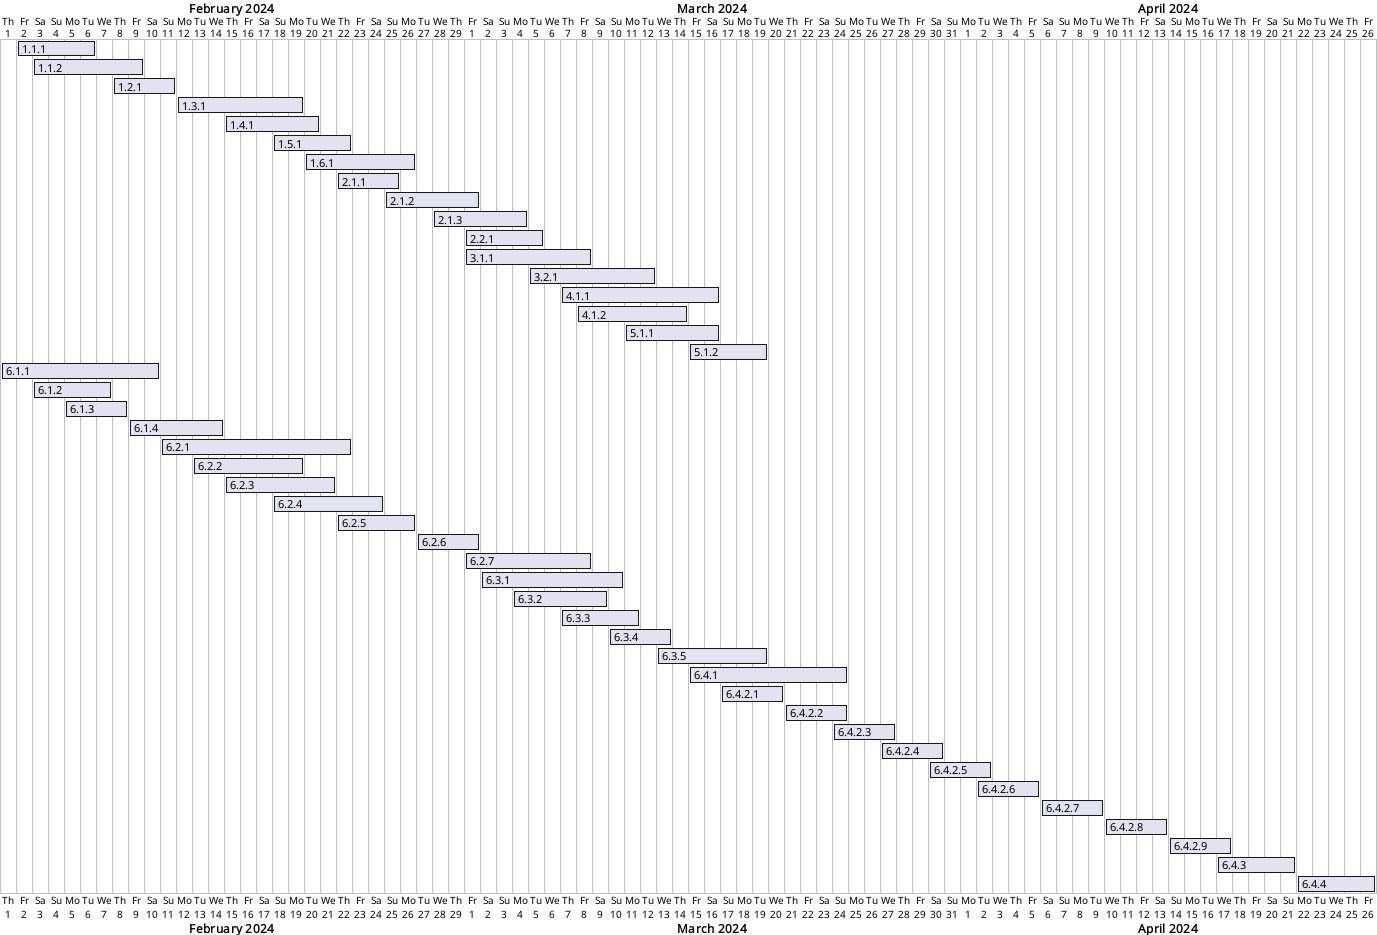
\includegraphics[height=\textwidth, angle=90]{figures/GANTT.png}
    \label{fig:gantt}
\end{figure}

\section{Terza Joint Project Planning Session}

\subsection{Agenda}

La terza Joint Project Planning Session è dedicata all'analisi dei rischi associati all'implementazione del progetto. L'agenda della riunione comprende:

\begin{itemize}
    \item Valutazione dei Rischi: Identificare e valutare i potenziali rischi che potrebbero influire sul raggiungimento degli obiettivi del progetto.
    \item Strategie di Mitigazione: Sviluppare strategie di mitigazione per affrontare i rischi individuati e ridurne l'impatto sul progetto.
\end{itemize}

\subsection{Deliverable}

I risultati della terza Joint Project Planning Session riflettono l'analisi dettagliata dei rischi, fornendo una base solida per la mitigazione dei rischi durante l'implementazione del progetto.

\subsubsection{Analisi dei rischi}

\paragraph{Rischi Tecnici:}

\begin{enumerate}
    \item \textbf{Scelta Tecnologica:}
          \begin{itemize}
              \item \textbf{Descrizione:} L'utilizzo di una nuova tecnologia potrebbe non portare agli obiettivi sperati o potrebbe non essere adatta.
              \item \textbf{Probabilità:} Media
              \item \textbf{Impatto:} Alto
              \item \textbf{Mitigazione:} Condurre una valutazione approfondita prima di adottare una nuova tecnologia. Effettuare test e prototipi per valutare l'efficacia della tecnologia.
          \end{itemize}

    \item \textbf{Complessità d'integrazione:}
          \begin{itemize}
              \item \textbf{Descrizione:} Problemi nella fase di integrazione dei vari componenti del sistema.
              \item \textbf{Probabilità:} Bassa
              \item \textbf{Impatto:} Medio
              \item \textbf{Mitigazione:} Pianificare test di integrazione regolari. Utilizzare standard aperti per facilitare l'interoperabilità.
          \end{itemize}
\end{enumerate}

\paragraph{Rischi di Project Management:}

\begin{enumerate}
    \item \textbf{Scarsa Organizzazione:}
          \begin{itemize}
              \item \textbf{Descrizione:} Una organizzazione inefficace può portare a ritardi e confusione.
              \item \textbf{Probabilità:} Media
              \item \textbf{Impatto:} Alto
              \item \textbf{Mitigazione:} Implementare metodologie di project management solide, assegnare chiaramente responsabilità e monitorare costantemente lo stato del progetto.
          \end{itemize}

    \item \textbf{Allocazione Inadeguata delle Risorse:}
          \begin{itemize}
              \item \textbf{Descrizione:} Risorse assegnate in modo inadeguato possono causare ritardi e sprechi.
              \item \textbf{Probabilità:} Media
              \item \textbf{Impatto:} Medio
              \item \textbf{Mitigazione:} Condurre un'analisi dettagliata delle risorse necessarie. Monitorare l'utilizzo delle risorse e adattare la pianificazione di conseguenza.
          \end{itemize}
\end{enumerate}

\paragraph{Rischi di Organizzazione:}

\begin{enumerate}
    \item \textbf{Priorità Maldefinite:}
          \begin{itemize}
              \item \textbf{Descrizione:} La mancanza di chiarezza sulle priorità può influenzare la direzione del progetto.
              \item \textbf{Probabilità:} Bassa
              \item \textbf{Impatto:} Medio
              \item \textbf{Mitigazione:} Stabilire chiaramente le priorità del progetto e comunicarle a tutti gli stakeholder. Mantenere una comunicazione aperta.
          \end{itemize}
\end{enumerate}

\paragraph{Rischi Esterni:}

\begin{enumerate}
    \item \textbf{Cambiamenti Normativi:}
          \begin{itemize}
              \item \textbf{Descrizione:} Modifiche nei requisiti legali e normativi possono influenzare il progetto.
              \item \textbf{Probabilità:} Bassa
              \item \textbf{Impatto:} Alto
              \item \textbf{Mitigazione:} Mantenere una stretta monitorazione degli sviluppi normativi. Adattare il progetto di conseguenza.
          \end{itemize}

    \item \textbf{Problemi con Fornitori:}
          \begin{itemize}
              \item \textbf{Descrizione:} Problemi con i fornitori possono causare ritardi nella fornitura di risorse o materiali.
              \item \textbf{Probabilità:} Media
              \item \textbf{Impatto:} Medio
              \item \textbf{Mitigazione:} Avere piani di contingenza per affrontare problemi con i fornitori. Mantenere una comunicazione chiara e regolare.
          \end{itemize}
\end{enumerate}